\documentclass[review]{elsarticle}

\usepackage{lineno,hyperref}
\modulolinenumbers[5]


%%%%%%%%%%%%%%%%%%%%%%%
%% Elsevier bibliography styles
%%%%%%%%%%%%%%%%%%%%%%%
%% To change the style, put a % in front of the second line of the current style and
%% remove the % from the second line of the style you would like to use.
%%%%%%%%%%%%%%%%%%%%%%%

%% Numberedo
%\bibliographystyle{model1-num-names}\usepackage{amssymb}



\usepackage{amssymb}
%\usepackage{amsmath}
\usepackage{pslatex}
\usepackage[overlap,CJK]{ruby}
\usepackage{linguex}
%\usepackage[pdftex]{graphicx}
\usepackage{graphicx}
\usepackage{multirow}
\usepackage{subfigure}
\usepackage{paralist}

\newcommand{\hlc}[2][yellow]{ {\sethlcolor{#1} \hl{#2}} }
\usepackage{fixltx2e}

\usepackage{tabularx}

\usepackage{dcolumn}
\usepackage{booktabs}
\usepackage{tikz}
\usetikzlibrary{positioning,shapes,arrows}

\newcolumntype{M}[1]{D{.}{.}{1.#1}}

%% Numbered without titles
%\bibliographystyle{model1a-num-names}

%% Harvard
%\bibliographystyle{model2-names.bst}\biboptions{authoryear}

%% Vancouver numbered
%\usepackage{numcompress}\bibliographystyle{model3-num-names}

%% Vancouver name/year
%\usepackage{numcompress}\bibliographystyle{model4-names}\biboptions{authoryear}

%% APA style
%\bibliographystyle{model5-names}\biboptions{authoryear}

%% AMA style
%\usepackage{numcompress}\bibliographystyle{model6-num-names}

%% `Elsevier LaTeX' style
\bibliographystyle{elsarticle-num}
%%%%%%%%%%%%%%%%%%%%%%%%

\begin{document}

\begin{frontmatter}

%\title{Combining Traditional Data Sources, Unmanned Aerial Vehicle Derived Data and Statistical Relational Learning to Improve Dengue Surveillance}

\title{Bayesian Prediction of Dengue Outbreaks Based on Disease Surveillance and Relational and  Meteorological Data}



\author[label1]{Raghvendra Jain}
\author[label2]{Sra  Sontisirikit}
\author[label3]{Sopon Iamsirithaworn}
\author[label4]{Marc Cavazza}
\author[label1]{Helmut Prendinger}

%\author[label3]{Klaus Br\"ugmann}

\address[label1]{{jain@nii.ac.jp, helmut@nii.ac.jp}\\
	National Institute of Informatics, \\
	2-1-2 Hitotsubashi, Chiyoda-ku, Tokyo, 101-8430, Japan\\}


\address[label2] {{arttioz@gmail.com} \\ 
	Asian Institute of Technology, School of Engineering and Technology, Thailand}

\address[label3]{{iamsiri@gmail.com}\\
	Department of Disease Control Thirteenth Division, Bangkok, Thailand}

\address[label4]{{M.O.Cavazza@kent.ac.uk} \\ 
	School of Engineering and Digital Arts, University of Kent} 



\begin{abstract}
To create early warning system of dengue outbreaks, we present a machine learning-based methodology capable of providing real-time (“nowcast”) and forecast estimates of dengue prediction in the Thailand by leveraging data from multiple data sources including: meteorological data, lag variables of disease surveillance, relational data of infected cases and  the data on spatial heterogeneity. Bayesian Network, a probabilistic graphical model was used to model causal relationships between the predictor variables and the dengue surveillance data.  \\
Our methodology enables...\\
We evaluate the predictive ability..\\
Our approach demonstrates several advantages: (1)...(2)..




%as outcome variable on the basis of data from 2001 to 2010. Data from 2011 to 2013 were used for external validation purposed of prediction accuracy of the model. Model fit were evaluated based on prediction performance in terms of detecting epidemics, and for number of predicted cases according to RMSE and SRMSE, as well as AIC. An optimal combination of meteorology and autoregressive lag terms of dengue counts in the past were identified best in predicting dengue incidence and the occurrence of dengue epidemics. Past data on disease surveillance, as predictor alone, visually gave reasonably accurate results for outbreak periods, but not for non-outbreaks periods. A combination of surveillance and meteorological data including lag patterns up to a few years in the past showed most predictive of dengue incidence and occurrence in Yogyakarta, Indonesia. The external validation showed poorer results than the internal validation, but still showed skill in detecting outbreaks up to two months ahead. Prior studies support the fact that past meteorology and surveillance data can be predictive of dengue. However, to a less extent has prior research shown how the longer-term past disease incidence data, up to years, can play a role in predicting outbreaks in the coming years, possibly indicating cross-immunity status of the population.


\textbf{Copied from PloS Paper}

Research is needed to create early warnings of dengue outbreaks to inform stakeholders and control the disease. This analysis composes of a comparative set of prediction models including only meteorological variables; only lag variables of disease surveillance; as well as combinations of meteorological and lag disease surveillance variables. Generalized linear regression models were used to fit relationships between the predictor variables and the dengue surveillance data as outcome variable on the basis of data from 2001 to 2010. Data from 2011 to 2013 were used for external validation purposed of prediction accuracy of the model. Model fit were evaluated based on prediction performance in terms of detecting epidemics, and for number of predicted cases according to RMSE and SRMSE, as well as AIC. An optimal combination of meteorology and autoregressive lag terms of dengue counts in the past were identified best in predicting dengue incidence and the occurrence of dengue epidemics. Past data on disease surveillance, as predictor alone, visually gave reasonably accurate results for outbreak periods, but not for non-outbreaks periods. A combination of surveillance and meteorological data including lag patterns up to a few years in the past showed most predictive of dengue incidence and occurrence in Yogyakarta, Indonesia. The external validation showed poorer results than the internal validation, but still showed skill in detecting outbreaks up to two months ahead. Prior studies support the fact that past meteorology and surveillance data can be predictive of dengue. However, to a less extent has prior research shown how the longer-term past disease incidence data, up to years, can play a role in predicting outbreaks in the coming years, possibly indicating cross-immunity status of the population.



\textbf{Our work}

To create early warning system of dengue outbreaks, we present a machine learning-based methodology capable of providing real-time (“nowcast”) and forecast estimates of dengue prediction in each of the fifty districts of Thailand by leveraging data from multiple data sources. Using a set of prediction variables we show an increasing prediction accuracy of the model with an optimal combination of predictors which include: meteorological data, clinical data, lag variables of disease surveillance, socio-economic data and the data  encoding spatial dependence on dengue transmission. We use generalized Generalized Additive Models (GAMs) to fit the relationships between the predictors and the clinical data of Dengue hemorrhagic fever (DHF) on the basis of the data from 2008 to 2012. Using the data from  2013 to 2015 and a comparative set of prediction models we evaluate the predictive ability of the fitted models according to RMSE and SRMSE, BIC as well as AIC. We also show that for the prediction of dengue outbreaks within a district, the influence of dengue incidences and socio-economic data from the surrounding districts is statistically significant, possibly indicating the influence of movement pattens of people and spatial heterogeneity of human activities on the spread of the epidemic.










%Our methodology exploits the information in each data source and produces accurate weekly predictions for up to four weeks ahead of the release of government reports. We evaluate the predictive ability of our ensemble approach during the 2013–2014 (retrospective) and 2014–2015 (live) flu seasons for each of the four weekly
%time horizons. 


%Our ensemble approach demonstrates several advantages: (1) our ensemble
%method’s predictions outperform every prediction using each data source independently,
%(2) our methodology can produce predictions one week ahead of GFT’s real-time
%estimates with comparable accuracy, and (3) our two and three week forecast estimates
%have comparable accuracy to real-time predictions using an autoregressive model. Moreover,
%our results show that considerable insight is gained from incorporating disparate data
%streams, in the form of social media and crowd sourced data, into influenza predictions in all
%time horizons.


\end{abstract}

\begin{keyword}
Dengue Forecasting \sep Statistical Relational learning \sep Probabilistic Relational Modeling \sep Bayesian Epidemiology \sep Disease Surveillance \sep Unmanned Aerial Vehicles. 
\end{keyword}

\end{frontmatter}

\linenumbers

\section{Introduction}

Dengue, a mosquito borne viral disease, has been a significant cause of death and hospitalization among children in developing countries such as India, Thailand etc. Despite this, the surveillance for diagnosing dengue has been limited which makes it difficult to generate detailed information on its epidemiology. The number of cases of dengue fever has increased dramatically since the 1960s, with between 50 and 528 million people infected yearly. Hundreds of thousands of cases of dengue are reported each year in tropical regions of the Americas, Africa, Asia, and Oceania. Globally, more than 2.5 billion people are at risk \cite{whodengue2012}. The World Health Organization (WHO) estimates that more than 50 million dengue virus (DENV) infections and 20,000 dengue disease-related deaths occur annually worldwide \cite{world2007scientific,whodengue2012fact}, and a recent disease distribution model estimated that were 390 million DENV infections in 2010, including 96 million apparent infections. Overall, 70\% of these apparent infections occurred in Asia \cite{bhatt2013global}. In 2015 alone, there were 111,826 reported cases in Thailand \cite{denguethai2015}. 

%Therefore, the goal of this research is to create a system that can acquire detailed relevant information and use it to predict the occurrence of dengue within a geographical region, so that public health experts can prepare for, manage and control the epidemic.  

%There are two main problems to realize the goal: \\
%\textbf{Problem 1:} \textit{Limitations of the method for data acquisition}. To understand the epidemiology of dengue, data about the changes in relevant environmental factors such as land usage pattern, radiation, toxins, pollutants, humidity, temperature etc., is required. However, the data acquired via satellite has several limitations e.g. infrequent data acquisition, higher operating cost, low spatial resolution (highest resolution is 41 cms), cloud contamination, required expertise for data management etc. Thus, the spatial and temporal accuracy of such data is limited. \\
%\textbf{Problem 2:} \textit{Limitations of the method of understanding epidemiology characteristic}. The hypothesis-testing methods such as national surveys and randomized controlled trials do not incorporate (2.a) high-dimensional longitudinal observational data (2.b) frequent updates of the variations in data (2.c) inherent uncertainties of the data sources, or (2.d) probabilistic relationship between ‘expected’ causes and effects of spread of dengue virus. 

%\texttt{To realize the goal, our approach is \textbf{probabilistic relational modeling of dengue epidemiology using UAV-derived data}. It has two goals to solve two corresponding problems 1 and 2: \\
%\textbf{Goal 1:} Data acquisition using unmanned aerial vehicles (UAVs). The use of UAVs overcomes the limitations associated with satellite data. Using UAVs enables (a) mounting onboard various sensors for different purposes (b) acquiring data with high spatial resolution (typically of 4-20 cms) in real-time and at frequent time points (c) ease-of-use without a significant training or technical knowledge (d) capturing of ‘stereo’ images that can be used for 3D visualization of the landscape and feature extraction. \\
%\textbf{Goal 2:} Understanding epidemiology using probabilistic relational models (PRMs). Unlike a BN, the PRM allows a more compact representation of domain of environmental impact assessment, which involves various factors, their attributes and relationships among them.}

%There have been numerous urban outbreaks of dengue with significant health and economic impact \cite{gubler2002epidemic,gubler2004cities,anuradha19981996,vaughn2000invited}. Studies in Thailand and Brazil have shown that the social and economic impact is equivalent to that of malaria in these countries \cite{clark2005economic,luz2009disability}. Dengue also poses a risk to those who travel to endemic areas and is increasingly being reported in travelers returning from trips to endemic countries \cite{farrar2007editorial}. However, globally, dengue research has not received the same level of funding as other tropical infectious diseases. 
%
%There are currently no available drugs and no licensed vaccine. The main mosquito control methodology: reducing the habitat and the number of mosquitoes and limiting exposure to bites is currently the best method for disease prevention. 


Thailand began to experience Dengue fever in 1949 and it became pandemic in the country for the first time in 1958 in Bangkok – Thonburi \cite{hammon1964virological}. Reports of clinically diagnosed cases of DF, DHF and DSS are compiled weekly at each hospital using a standard form containing essential patient information. These are then sent to the Provincial Health Offices who undertake local control measures and subsequently forward the information to the Epidemiology Department in Bangkok \cite{chareonsook1999changing}. The situation of dengue fever since the year 1958 -2015 are likely to rise \cite{wilder2012denguetools}. Most patients are in 0-14 age group, the highest incidence rate in the age group 5-9 years, the ratio of female to male patients is similar \cite{cummings2009impact,wilder2012denguetools}. 


There are four distinct, but closely related, serotypes of the virus that cause dengue (DEN-1, DEN-2, DEN-3 and DEN-4) \cite{gubler1995dengue,whodenvtype2015}. Recovery from infection by one provides lifelong immunity against that particular serotype. However, cross-immunity to the other serotypes after recovery is only partial and temporary (6-12 months) \cite{gubler1995dengue}. Subsequent infections by other serotypes increase the risk of developing severe dengue. Once infected, humans become the main carriers and multipliers of the virus, serving as a source of the virus for uninfected mosquitoes. The virus circulates in the blood of an infected person for 2-7 days, at approximately the same time that the person develops a fever. Patients who are already infected with the dengue virus can transmit the infection via Aedes mosquitoes after the first symptoms appear (during 4-5 days; maximum 12) \cite{whodenvsym2015}.

Symptoms, which usually begin four to six days after infection and last for up to 10 days, may include: sudden high fever, severe headaches, pain behind the eyes, severe joint and muscle pain, fatigue, nausea, vomiting, skin rash (which appears two to five days after the onset of fever) and mild bleeding (such a nose bleed, bleeding gums, or easy bruising) Sometimes, symptoms are mild and can be mistaken for those of the flu or another viral infection. Younger children and people who have never had the infection before tend to have milder cases than older children and adults. However, serious problems can develop. These include dengue hemorrhagic fever, a rare complication characterized by high fever, damage to lymph and blood vessels, bleeding from the nose and gums, enlargement of the liver, and failure of the circulatory system. The symptoms may progress to massive bleeding, shock, and death. This is called dengue shock syndrome (DSS) \cite{webmdsymptoms2015}. 

Transmission of DENV has increased dramatically in the past two decades, making DENV one of the most important human pathogens among arthropod-borne viruses \cite{hesse2007dengue}. Moreover, There are currently no licensed vaccines or specific therapeutics, and substantial vector control efforts have not stopped its rapid emergence and global spread \cite{tatem2006global}. About 50-100 million dengue fever infections occur every year in tropical and subtropical countries\cite{gubler2002epidemic}.  The infection by one type usually gives lifelong immunity to that type, but only short-term immunity to the others. Transmission occurs through the bite of infected Aedes mosquitoes, principally Aedes aegypti. This kind of mosquito prefers to breed in areas of stagnant water, such as flower vases, uncovered barrels, buckets, and discarded tires, but the most dangerous areas are wet shower floors and toilet tanks, as they allow the mosquitoes to breed inside the residence. Flight range studies suggest that most female Aedes mosquito may spend their lifetime in or around the houses where they emerge as adults and they usually fly an average of 400 metres \cite{whomosquito2007}. Although the lifespan of an adult Aedes mosquito is two to four weeks depending on conditions \cite{zettel2012yellow}, the eggs can be viable for over a year in a dry state, which allows the mosquito to re-emerge after a cold winter or dry spell \cite{mortimer1998aedes}.

 

There have been numerous urban outbreaks of dengue with significant health and economic impact \cite{gubler2002epidemic,gubler2004cities,anuradha19981996,vaughn2000invited}. Studies in Thailand and Brazil have shown that the social and economic impact is equivalent to that of malaria in these countries \cite{clark2005economic,luz2009disability}. Therefore, the goal of this research is to create a system that can acquire detailed relevant information and use it to predict the occurrence of dengue within a geographical region, so that public health experts can prepare for, manage and control the epidemic.  




%
%There are currently no available drugs and no licensed vaccine. The main mosquito control methodology: reducing the habitat and the number of mosquitoes and limiting exposure to bites is currently the best method for disease prevention. 
	
	
%This research will focus on analyzing captured data from UAVs sensors such as image to classified land-type, landmark, and weather for estimating infection factors from Aedes mosquito combined with population statistics in the target area to predict risk of dengue outbreak.
%	\begin{figure}[htbp]
%		\begin{center}
%			\includegraphics[width=150mm]{./figures/denguespread}
%			\caption[Increase of dengue incidence rate from 1970-2007 in worldwide. Reprinted from the website of \protect\cite{whoimpactdengue2008}.]{The figure show the increase of incidence rate of dengue from 1970-2007. Before 1970, there are only 9 countries that experienced DHF cases. But in twenty-first century, the incident rate is increase dramatically and the disease is now endemic in more than 100 countries. Up to 50 million infections occur annually with 500 000 cases of DHF and 22,000 deaths mainly among children. The virus became the most important mosquito-borne viral disease in the world. Reprinted from the website of \protect\cite{whoimpactdengue2008}.}	
%			\label{figure-denguespread}
%		\end{center}
%	\end{figure}
%	%----------------------------------------------------------------------------------------------------------------------------------------------------------------------------------------
%\section{Problem Statement}


The risk of epidemic dengue transmission is determined by a combination of factors that include level of human immunity to virus serotypes, virulence characteristics of the virus strain, abundance of Aedes mosquitoes, weather, and population statistics in target area \cite{focks1995simulation}. Several potential predictive indicators for outbreaks have been described\cite{leitmeyer1999dengue,runge2008does,thammapalo2008environmental,sarfraz2014near}. There are several  environmental factors related to dengue outbreak that have been identified from case studies in Southeast Asia \cite{sulaiman1996relationship,thammapalo2008environmental,sarfraz2014near,nakhapakorn2005information}. There are many research conclude that most dengue cases are occurred in urban areas due to various contributing factors such high population density, inadequate housing, and inappropriate human behavioral practices \cite{chang2009combining,knudsen1992vector,troyo2009urban}.  Surveillance of Aedes mosquito density is important for construction models of dengue transmission, in order to prioritize areas and seasons for vector control. The 80\% of larvae or pupa in house are from Aedes mosquito. \cite{sarfraz2014near} extract land-use types using object-based and spatial metric approaches to explore dengue incidence in relation to the surrounding environment in near real-time using Google and Advanced Land Observation Satellite images. Geospatial analysis on public health data indicated that most of the dengue cases were found in densely populated areas \textit{surrounded by dense vegetation}. Dense vegetation can facilitate the invasion of Aedes mosquitoes by providing abundant resting sites. 

The empirical relationship of climatic factors rainfall, temperature and humidity with the DF/DHF incidences has been studied \cite{nakhapakorn2005information, li1985rainfall,hales2002potential,rueda1990temperature,tun2000effects,brady2013modelling}.  According to the development period from a mosquito egg to the human disease, there is a time lag of about one month that leads to DF/DHF cases occurring in 7 - 45 days. Thus, DF/DHF cases at time t (in month e.g. May) depend on others factors at time t-1 (i.e. one month before month) as validated in the empirical analysis \cite{nakhapakorn2005information}. The diurnal temperature range (DTR) is the difference between the daily maximum and minimum temperature. The experimental evaluation shows that DTR affects two important parameters underlying dengue virus (DENV) transmission by Aedes mosquito \cite{lambrechts2011impact}. 


	
%\section{Objectives}
	
%We study the environmental factors of dengue fever outbreak from dengue patients recoded data in Bangkok, Thailand. These data of each patient which can be used to study geographic factors related to dengue fever by mapping address locations to satellite imagery, then analyzing the common landmarks and land types that close to outbreak locations. The mosquito population is also highly dependent on climate.  In order to tackle this issues, we will need to divided the data in to set divided by district area. The analyzed data will be used to train and test for the prediction model. The second step of the project will be to identify  environmental factors that can be observed locally by a UAVs that are pertinent in the context of dengue. Some of the indices that we would like to study include: number of suspect areas that have Aedes mosquito lairs, humidity, air warmness, density of houses, quality of houses, level of precipitation, and so on. 
%In this research we: 
%	
%	\begin{enumerate}
%		\item Identify the environmental factors of dengue fever by environments of patient’s house and UAVs sensor data.
%		
%		\item Analyze the causes and consequences of existing dengue fever factors to calculate the possibility of dengue fever outbreaks in target area. 
%		
%		\item Build a new prototype system able to integrate data from multiple sensor platforms and data sources in order to measure the inputs to the model describes in objective above automatically. 
%		
%		\item Evaluate of the prototype combined with prediction model by surveying one village in Bangkok.
%	\end{enumerate}
	
	%----------------------------------------------------------------------------------------------------------------------------------------------------------------------------------------




\section{Materials and Methods}

\subsection{Study area}
\label{section-study-area}

The dengue outbreak in Bangkok can affect to dengue situation for the whole country, because Bangkok is a very crowded city  locate at the center part of Thailand. In the 2010 census, Bangkok had a population of 8.28 million, although just 5.7 million were registered residents. Much of the daytime population commutes from surrounding areas in the region, bringing the total population to 15 million \cite{WPR2015}. During winter season, temperature in Bangkok still high around 28-35 degree Celsius and there is rain in every season \cite {wwo2012}. %Figures \ref{figure-avg_temp_bangkok} and \ref{figure-avg_rain_bangkok} show the average temperature and rain of the Bangkok. 
This makes the city is very suitable for Aedes mosquito to breeding making dengue virus spread from  Bangkok in every season. Moreover, many people who live in Bangkok travel to other provinces frequently, so these people may be the main carriers and multipliers of the virus that cause dengue outbreak in other part of Thailand. Figure \ref{figure-dengue_incident_rate} shows the relationship between incidences of dengue per one hundred thousand people in Thailand versus Bangkok. The dengue incident rate in Bangkok is nearly the same as the whole country. So, if we could reduce dengue incident rates in Bangkok, the rate in Thailand will be reduce too because there will be fewer dengue carriers who travel from Bangkok to other parts of Thailand.

%\begin{figure}[htbp]
%	\begin{center}
%		\includegraphics[width=145mm]{./figures/avg_temp_bangkok}
%		\caption{Average high and low temperature in Bangkok from 2000-2012. Reprinted from \protect\cite{wwo2012}.}
%		\label{figure-avg_temp_bangkok}
%	\end{center}
%\end{figure}
%
%\begin{figure}[htbp]
%	\begin{center}
%		\includegraphics[width=145mm]{./figures/avg_rain_bangkok}
%		\caption{Average rainfall in Bangkok from 2000-2012. Reprinted from \protect\cite{wwo2012}.}
%		\label{figure-avg_rain_bangkok}
%	\end{center}
%\end{figure}



\begin{figure}[htbp]
	\begin{center}
		\includegraphics[width=140mm]{./figures/dengue_incident_rate}
		\caption{ Relationship between incidences of dengue per one hundred thousand people in Thailand versus Bangkok from 2005 - 2014.}
		\label{figure-dengue_incident_rate}
	\end{center}
\end{figure}

% 3.1.1
%\subsection{Bangkok districts}

%The Bangkok city covers an area of 1,568.737 square kilometres and it is subdivided into 50 districts , which are further subdivided into 169 sub-districts. Total population who registered in Bangkok is 5,693,884 and more than three million people are live in Bangkok without registered. Table \ref{table-bangkok-district} and figure \ref{figure-bangkok_district} show district name, map and population statistic in each area. The average registered population of Bangkok districts in 2014 is 113845. The highest population district is Saimai (194,511) and the lowest population district is Samphanthawongse (26359). But the highest and lowest population density district are Phranakhon (157791 men/km 2) and Thawiwatthana (2948 men/km 2).  Data of Bangkok statistics described more later in subsection "Prediction variable".

%\begin{table}[htbp]
%	\centering
%	\scriptsize
%	\label{table-bangkok-district}
%	\resizebox{1.2\textwidth}{!}{
%	\begin{tabular}{|l|l|l|l|l|}
%		\hline
%		ID Map & District Name & Population & Area  & Density\\
%		\hline
%		1 & Phranakhon & 55373 & 5.536 & 157791\\
%		\hline
%		2 & Bangbon & 107140 & 34.745 & 3084\\
%		\hline
%		3 & Chomthong & 156030 & 26.265 & 28111\\
%		\hline
%		4 & Bangrak & 46472 & 5.536 & 42529\\
%		\hline
%		5 & Bangkhae & 191966 & 44.456 & 18428\\
%		\hline
%		6 & Bangkapi & 148964 & 28.523 & 10853\\
%		\hline
%		7 & Patumwan & 51557 & 8.369 & 28172\\
%		\hline
%		8 & Pom prap & 49280 & 1.931 & 127030\\
%		\hline
%		9 & Prakanong & 92448 & 13.986 & 6610\\
%		\hline
%		10 & Minburi & 139771 & 63.645 & 4619\\
%		\hline
%		11 & Don muang & 168197 & 36.803 & 14759\\
%		\hline
%		12 & Yannawa & 80843 & 16.662 & 9651\\
%		\hline
%		13 & Samphanthawongse & 26359 & 1.416 & 55837\\
%		\hline
%		14 & Payathai & 72203 & 9.595 & 7525\\
%		\hline
%		15 & Thung khru & 119349 & 30.741 & 7861\\
%		\hline
%		16 & Bangkok yai & 70003 & 6.18 & 27711\\
%		\hline
%		17 & Huai khwang & 80002 & 15.033 & 16746\\
%		\hline
%		18 & Thawiwatthana & 77121 & 50.219 & 2948\\
%		\hline
%		19 & Taling chan & 105857 & 29.479 & 26455\\
%		\hline
%		20 & Suanluang & 118371 & 23.678 & 4999\\
%		\hline
%		21 & Lat Krabang  & 168309 & 123.859 & 10304\\
%		\hline
%		22 & Dindaeng & 127260 & 8.354 & 15233\\
%		\hline
%		23 & Nongkhaem & 153175 & 35.825 & 8572\\
%		\hline
%		24 & Radburana & 84881 & 15.782 & 10678\\
%		\hline
%		25 & Bangplad & 96787 & 11.36 & 34173\\
%		\hline
%		26 & Bangsue & 128995 & 11.545 & 22359\\
%		\hline
%		27 & Bung kum & 145514 & 24.311 & 17772\\
%		\hline
%		28 & Watthana & 83520 & 12.565 & 18145\\
%		\hline
%		29 & Pasricharoen & 129238 & 17.834 & 51163\\
%		\hline
%		30 & Prawet & 166364 & 52.49 & 9346\\
%		\hline
%		31 & Saphansung & 92735 & 28.124 & 3297\\
%		\hline
%		32 & Nong chokn & 162598 & 236.261 & 5799\\
%		\hline
%		33 & Klongtoey & 107221 & 12.994 & 22270\\
%		\hline
%		34 & Thon buri & 115330 & 8.551 & 98020\\
%		\hline
%		35 & Jatujak & 160366 & 32.908 & 26676\\
%		\hline
%		36 & Bangkuntien & 173144 & 120.687 & 3940\\
%		\hline
%		37 & Ratchathervi & 73790 & 7.126 & 41593\\
%		\hline
%		38 & Lat Phrao & 122196 & 22.157 & 10180\\
%		\hline
%		39 & Sathorn & 82432 & 9.326 & 28089\\
%		\hline
%		40 & Saimai & 194511 & 44.615 & 13386\\
%		\hline
%		41 & Laksi & 107797 & 22.841 & 9472\\
%		\hline
%		42 & Bangkhen & 190659 & 42.123 & 9221\\
%		\hline
%		43 & Kannayao & 92094 & 25.98 & 7086\\
%		\hline
%		44 & Bang kholam & 92273 & 10.921 & 28042\\
%		\hline
%		45 & Wang thonglang & 114245 & 19.265 & 24568\\
%		\hline
%		46 & Klongsamwa & 178958 & 110.686 & 8751\\
%		\hline
%		47 & Bangna & 94315 & 18.789 & 5020\\
%		\hline
%		48 & Klongsan & 75224 & 6.051 & 54926\\
%		\hline
%		49 & Bangkok noi & 116653 & 11.944 & 52187\\
%		\hline
%		50 & Dusit & 104394 & 10.665 & 58514\\
%		\hline
%	\end{tabular}
%}
%	\caption{Bangkok district population in 2014. Density is number of people per km$^{2}$. Data from Department of Provincial Administration, Ministry of Interior, Thailand }
%\end{table}



%\begin{figure}[htbp]
%	\begin{center}
%		\includegraphics[width=140mm]{./figures/bangkok_district}
%		\caption{ Bangkok districts, Reprinted from \protect\cite{wikibangkok}.}
%		\label{figure-bangkok_district}
%	\end{center}
%\end{figure}

% 3.1.2
%\subsection{Dengue fever in Bangkok district}


Figure \ref{figure-bangkok-data} (a) shows the increase of dengue cases in Bangkok up to 2015. The average number of dengue cases in Bangkok from 2005 until 2015 is around 10,758 cases per year. The highest number of dengue cases in Bangkok is 28,177 cases which happened in 2015. Figure \ref{figure-bangkok-data} (b) shows changes in dengue serotypes from 2005 to 2015. The percentage of dengue serotypes DENV 1 - 4 in the central part of Thailand changed every year, making people who already have immunity to one serotype susceptible to infection with another serotype in the following year. Figure \ref{figure-dengue_bangkok_2015} shows the effect of season on dengue cases. In rain season (mid May - October), dengue cases rise dramatically, and then they decrease suddenly in summer season (February - mid May). The reason that November has the highest number cases is that dengue virus in patients need 4 - 10 days for the incubation period. So most dengue patients in November are infected in rain season (October).  


\begin{figure}[htbp]
	\begin{center}
		\includegraphics[width=145mm]{./figures/bangkok_dengue_data}
		\caption{ (a) Dengue cases from 2010 - 2015 in Bangkok. (b) Dengue serotypes from 2005 - 2010 in central Thailand. Data from Department of Disease Control 13th Division and \protect\cite{limkittikul2014epidemiological}. }
		\label{figure-bangkok-data}
	\end{center}
\end{figure}


\begin{figure}[htbp]
	\begin{center}
		\includegraphics[width=120mm]{./figures/dengue_bangkok_2015}
		\caption{ Monthly dengue cases in Bangkok  2015. Data from Department of Disease Control 13th Division. }
		\label{figure-dengue_bangkok_2015}
	\end{center}
\end{figure}




\subsection{Prediction variable and data collection}
\label{section-Prediction-variable}

There are three main factors that affect to dengue incidence cases: other cases of dengue virus, presence of Aedes mosquitoes, and various human factors. Dengue fever cannot spread to humans from other animal; mosquitoes are mainly carries. Typically, people infected with dengue virus are asymptomatic (80\%) or have only mild symptoms , such as an uncomplicated fever \cite{whitehorn2010dengue,reiter2010yellow}. In Bangkok's case, dengue fever and dengue hemorrhagic fever were reported in each season,  mean, dengue virus  is always present in human too. Once infected, \textit{humans} become the main carriers and multipliers of the virus, serving as a source of the virus for uninfected \textit{Aedes mosquitoes} to carry. 

\begin{enumerate}
	\item Dengue virus prediction variable:
	\begin{itemize}
		\item \textbf{Monthly DF/DHF incidents in the district} represents the number of dengue virus report in the target district. 
		\item  \textbf{Monthly DF/DHF incident in the nearby districts} represents the number of dengue virus reports which may affect to the target district
	\end{itemize}
	\item Aedes mosquito prediction variables
		\begin{itemize}
			\item  \textbf{Monthly rainfall in district} represents the density of Aedes mosquitoes in the target district. 
			\item \textbf{Monthly average diurnal temperature range (DTR) in Bangkok} represents the health of the dengue virus in Aedes mosquito. Higher DTR means  lower health of dengue virus in Aedes mosquito, deceasing infection rates.
		\end{itemize}
	\item Human prediction variables
		\begin{itemize}
				\item \textbf{Population with age less than 35 in the district} represents the proportion of the district population that has a high risk for dengue fever. 
				
				\item \textbf{Population age 35+ in the district} represents the proportion of the district population that has a low risk for dengue fever.
				
				\item \textbf{Annual population density in district} represents how easy to transmit dengue virus from one person other other person by Aedes mosquito. 
				
				\item \textbf{Number of communities  in  the district} represents how large the group are, make it more of less convenient transmission of dengue virus by Aedes mosquito.
		\end{itemize}
\end{enumerate}



%The analysis of dengue case data and human prediction variable in Bangkok in Microsoft Excel. I determined the relationship between average dengue incidence rate from 2005-2015 and the number of communities in each individual district. Figure \ref{figure-dengue_community_vs_cases} shows that fewer communities district may have higher dengue than district with a large number of communities.
%
%
%\begin{figure}[htbp]
%	\begin{center}
%		\includegraphics[width=120mm]{./figures/dengue_community_vs_cases}
%		\caption{ Average dengue rates per 100,00 people from 2005-2015 and number of communities in individual district of Bangkok.  Dengue cases data from Department of Disease Control 13th division and Community data from Department of Social Development, Bangkok.}
%		\label{figure-dengue_community_vs_cases}
%	\end{center}
%\end{figure}



\subsubsection{Analysis Using Bayesian network model}
\label{section-bayesian-network-model}

Figure \ref{figure-bn_md_dr} depicts the directed acyclic graph for the Bayesian network, and table \ref{table-bn-md-dag} describes the conditional probability distributions of variables in model.

\begin{table}[!htbp]
		\centering
		\normalsize
%		\resizebox{1.4\textwidth}{!}
     \resizebox{1.2\textwidth}{!}{
		\begin{tabular}{|l|p{2cm}|l|l|} 
			\hline
			Name & Abbreviation & Predict possibilities output & Parents (Pa)\\
			\hline
			Mosquito density & MD &  $MD_0$: Low &  Outside house breeding container\\
			&  &  $MD_1$: Moderate &  Inside house breeding container\\
			&  &  $MD_2$: High &  Diurnal temperature range\\
			\hline
			Outside house breeding container & OB &  $OB_0$:Low &  Neglect garbage\\
			&  &  $OB_1$:High &  Rain\\
			\hline
			Inside house breeding container & IB &  $IB_0$:Low &  Cleaning activity\\
			&  &  $IB_1$:High &  House type \\
			\hline
			Neglect garbage & NG &  $NG_0$:Low &  Cleaning activity\\
			&  &  $NG_1$:High &  Population density\\
			\hline
			Cleaning activity & CA &  $CA_0$:Low &  Awareness \\
			&  &  $CA_1$:High & \\
			\hline
			Rain & R &  $R_1$:Low &  Season \\
			&  &  $R_1$:Moderate & \\
			&  &  $R_2$:High & \\
			\hline
			Diurnal temperature range & DTR &  $DTR_0$:Low &  Season \\
			&  &  $DTR_1$:High & \\
			\hline
			House Density & HT &  $HT_0$:Low & \\
			&  &  $HT_1$:High & \\
			\hline
			Awareness & A &  $A_0$:Low & \\
			&  &  $A_1$:High & \\
			\hline
			Season & S &  $S_0$:Summer & \\
			&  &  $S_1$:Winter & \\
			&  &  $S_2$:Rain & \\
			\hline
			Population density & PD & $PD_0$:Low & \\
			&  &  $PD_1$:High & \\
			\hline
		\end{tabular}
	}
		\caption{Notation of the variables used in Bayesian network model}
		\label{table-bn-md-dag}
	\end{table}


\begin{table}[!htbp]
		\centering
		\normalsize
		\begin{tabular}{|l|l|l|l|l|l|}
			\hline
			\multicolumn{3}{|l|}{Pattern}	 & P( $MD_0$ $\mid$ PA) & P($MD_1$ $\mid$ PA) & P($MD_2$  $\mid$ PA)\\
			\hline
			$OB_0$ & $IB_0$ & $DTR_0$ & 1 & 0 & 0\\
			\hline
			$OB_0$ & $IB_0$ & $DTR_1$ & 1 & 0 & 0\\
			\hline
			$OB_0$ & $IB_1$ & $DTR_0$ & 0 & 0.7 & 0.3\\
			\hline
			$OB_0$ & $IB_1$ & $DTR_1$ & 0.2 & 0.6 & 0.2\\
			\hline
			$OB_1$ & $IB_0$ & $DTR_0$ & 0 & 0.3 & 0.7\\
			\hline
			$OB_1$ & $IB_1$ & $DTR_0$ & 0 & 0 & 1\\
			\hline
			$OB_1$ & $IB_0$ & $DTR_1$ & 0 & 0.5 & 0.5\\
			\hline
			$OB_1$ & $IB_1$ & $DTR_1$ & 0 & 0 & 1\\
			\hline
		\end{tabular}
		\caption{ Conditional probability distribution of mosquito density}
		\label{condition-md}
	\end{table}
	
	
	\begin{table}[!htbp]
		\centering
		\normalsize
		\begin{tabular}{|l|l|l|l|}
			\hline
			\multicolumn{2}{|l|}{Pattern}  & P(OB0 $\mid$ PA) & P(OB1 $\mid$ PA)\\
			\hline
			$NB_0$ & $R_0$ & 1 & 0\\
			\hline
			$NB_0$ & $R_1$ & 0.4 & 0.6\\
			\hline
			$NB_0$ & $R_2$ & 0.2 & 0.7\\
			\hline
			$NB_1$ & $R_0$ & 0.9 & 0.1\\
			\hline
			$NB_1$ & $R_1$ & 0.2 & 0.8\\
			\hline
			$NB_1$ & $R_2$ & 0 & 1\\
			\hline
		\end{tabular}
		\caption{Conditional probability distribution of density of outside house breeding spot}
		\label{condition-ob}
	\end{table}
	
	\begin{table}[!htbp]
		\centering
		\normalsize
		\begin{tabular}{|l|l|l|l|}
			\hline
			\multicolumn{2}{|l|}{Pattern}  & P(IB0 $\mid$ PA) & P(IB1$\mid$ PA)\\
			\hline
			CA0 & HT0 & 0.6 & 0.4\\
			\hline
			CA0 & HT1 & 0 & 1\\
			\hline
			CA1 & HT0 & 1 & 0\\
			\hline
			CA1 & HT1 & 0.4 & 0.6\\
			\hline
		\end{tabular}
		\caption{Conditional probability distribution of density of inside house breeding container}
		\label{condition-ib}
	\end{table}
	
	\begin{table}[!htbp]
		\centering
		\normalsize
		\begin{tabular}{|l|l|l|l|}
			\hline
			\multicolumn{2}{|l|}{Pattern}  & P(NG0 $\mid$ PA) & P(NG1 $\mid$ PA)\\
			\hline
			CA0 & PD0 & 0.4 & 0.6\\
			\hline
			CA0 & PD1 & 0 & 1\\
			\hline
			CA1 & PD0 & 0.9 & 0.1\\
			\hline
			CA1 & PD1 & 0.6 & 0.4\\
			\hline
		\end{tabular}
		\caption{Conditional probability distribution of neglect garbage}
		\label{condition-grb}
	\end{table}
	
	\begin{table}[!htbp]
		\centering
		\normalsize
		\begin{tabular}{|l|l|l|}
			\hline
			Pattern & P(CA0 $\mid$ PA) & P(CA1 $\mid$ PA)\\
			\hline
			A0 & 1 & 0\\
			\hline
			A1 & 0 & 1\\
			\hline
		\end{tabular}
		\caption{Conditional probability distribution of cleaning activity}
		\label{condition-ca}
	\end{table}
	
	
	\begin{table}[!htbp]
		\centering
		\normalsize
		\begin{tabular}{|l|l|l|l|}
			\hline
			Pattern & P(R0 $\mid$ PA) & P(R1 $\mid$ PA) & P(R2 $\mid$ PA)\\
			\hline
			S0 & 1 & 0 & 0\\
			\hline
			S1 & 0.4 & 0.6 & 0\\
			\hline
			S2 & 0 & 0.2 & 0.8\\
			\hline
		\end{tabular}
		\caption{Conditional probability distribution of rain}
		\label{condition-rain}
	\end{table}
	
	\begin{table}[!htbp]
		\centering
		\normalsize
		\begin{tabular}{|l|l|l|}
			\hline
			Pattern & P(DTR0 $\mid$  PA) & P(DTR1 $\mid$  PA)\\
			\hline
			S0 & 0 & 1\\
			\hline
			S1 & 1 & 0\\
			\hline
			S2 & 0.9 & 0.1\\
			\hline
		\end{tabular}
		\caption{Conditional probability distribution of Diurnal temperature range}
		\label{condition-dtr}
	\end{table}
	
	\begin{table}[!htbp]
		\centering
		\normalsize
		\begin{tabular}{|l|l|l|l|}
			\hline
			Name & Abbreviation & Predict possibilities output & Parents (Pa)\\
			\hline
			Actual report & ARDC & ARDC0:Under report &  Hospital Awareness \\
			DF/DHF Cases &  & ARDC1:Moderate report &  Dengue rate\\
			&  & ARDC2:Active report & \\
			\hline
			Dengue rate & DR & DR0:Low &  Infected Mosquitos \\
			&  & DR1:Moderate &  Immune Dengue People\\
			&  & DR2:High & \\
			\hline
			Density of infected Mosquitos & IM & IM0:Low  &  Dengue Cases \\
			&  & IM0:Moderate &  Dengue Case of nearby district\\
			&  & IM1:High &  Diurnal temperature range\\
			&  &  &  Mosquito density\\
			\hline
			Immune Dengue People & IP & IP0:Low &  Dengue Cases \\
			&  & IP1:Moderate & \\
			&  & IP2:High & \\
			\hline
			Diurnal temperature range & DTR & DTR0:Low &  Season \\
			&  & DTR1:High & \\
			\hline
			Dengue Cases & DC & DC0:Low & \\
			&  & DC1: Moderate & \\
			&  & DC2:High & \\
			\hline
			Dengue Case of nearby district & DCN & DCN0:Low & \\
			&  & DCN1: Moderate & \\
			&  & DCN2:High & \\
			\hline
			Mosquito density & MD & MD0: Low & \\
			&  & MD1: Moderate & \\
			&  & MD2: High & \\
			\hline
			Hospital Awareness & HA & HA0: Low & \\
			&  & HA1: High & \\
			\hline
			Population Density & PD & PD0: Low & \\
			&  & PD1: High & \\
			\hline
			Season & S & ·      S0:Summer & \\
			&  & ·      S1:Winter & \\
			&  & ·      S2:Rain & \\
			\hline 
			Awareness & A & ·      A0:Low & \\			
			&  & ·      A1:High & \\
			\hline
			
		\end{tabular}
		\caption{Notation of the variables used in Bayesian network model}
		\label{notation-bn2}
	\end{table}
	
	\begin{table}[!htbp]
		\centering
		\normalsize
		\begin{tabular}{|l|l|l|l|l|}
			\hline
			\multicolumn{2}{|l|}{Pattern}  & P(ARDC 0 $\mid$ PA) & P(ARDC 1 $\mid$ PA) & P(ARDC2 $\mid$ PA)\\
			\hline
			HA0 & DR0 & 1 & 0 & 0\\
			\hline
			HA0 & DR1 & 0.7 & 0.2 & 0.1\\
			\hline
			HA0 & DR2 & 0.3 & 0.5 & 0.2\\
			\hline
			HA1 & DR0 & 0.7 & 0.3 & 0\\
			\hline
			HA1 & DR1 & 0.3 & 0.5 & 0.2\\
			\hline
			HA1 & DR2 & 0 & 0.2 & 0.8\\
			\hline
		\end{tabular}
		\caption{Conditional probability distribution of Actual report DF/DHF Cases}
	    \label{condition-dh}
	\end{table}
	
	\begin{table}[!htbp]
		\centering
		\normalsize
		\begin{tabular}{|l|l|l|l|l|}
			\hline
			\multicolumn{2}{|l|}{Pattern}   & P(DR0 $\mid$  PA) & P(DR 1 $\mid$  PA) & P(DR 2 $\mid$  PA)\\
			\hline
			IM0 & IP x & 1 & 0 & 0\\
			\hline
			IM1 & IP 0 & 0 & 0.3 & 0.7\\
			\hline
			IM1 & IP 1 & 0.1 & 0.4 & 0.5\\
			\hline
			IM1 & IP 2 & 0.1 & 0.5 & 0.4\\
			\hline
			IM2 & IP 0 & 0 & 0 & 1\\
			\hline
			IM2 & IP 1 & 0 & 0.1 & 0.9\\
			\hline
			IM2 & IP 2 & 0 & 0.3 & 0.7\\
			\hline
		\end{tabular}
		\caption{Conditional probability distribution of dengue incident rate (DF/DHF cases)}
		\label{condition-rdh}
	\end{table}
	
	\begin{table}[!htbp]
		\centering
		\normalsize
		\begin{tabular}{|l|l|l|l|}
			\hline
			Pattern & P(IP0 $\mid$ PA) & P(IP1 $\mid$ PA) & P(IP2 $\mid$ PA)\\
			\hline
			DC0 & 1 & 0 & 0\\
			\hline
			DC1 & 0 & 1 & 0\\
			\hline
			DC2 & 0 & 0 & 1\\
			\hline
		\end{tabular}
		\caption{Conditional probability distribution of immune dengue people}
		\label{condition-idp}
	\end{table}
	
	\begin{table}[!htbp]
		\centering
		\normalsize
		\begin{tabular}{|l|l|l|l|l|l|l|}
			\hline
			\multicolumn{4}{|l|}{Pattern}    & P(IM0 $\mid$ PA) & P(IM1 $\mid$ PA) & P(IM2 $\mid$ PA)\\
			\hline
			DC0 & DCN 0 & MD0 & DTRx & 1 & 0 & 0\\
			\hline
			DC0 & DCN 0 & MD1 & DTRx & 0.9 & 0.1 & 0\\
			\hline
			DC0 & DCN 0 & MD2 & DTR0 & 0.7 & 0.3 & 0\\
			\hline
			DC0 & DCN 0 & MD2 & DTR1 & 0.8 & 0.2 & 0\\
			\hline
			DC0 & DCN 1 & MD0 & DTRx & 1 & 0 & 0\\
			\hline
			DC0 & DCN 1 & MD1 & DTR0 & 0.7 & 0.3 & 0\\
			\hline
			DC0 & DCN 1 & MD1 & DTR1 & 0.8 & 0.2 & 0\\
			\hline
			DC0 & DCN 1 & MD2 & DTR0 & 0.3 & 0.7 & 0\\
			\hline
			DC0 & DCN 1 & MD2 & DTR1 & 0.4 & 0.6 & 0\\
			\hline
			DC0 & DCN 2 & MD0 & DTRx & 0.9 & 0.1 & 0\\
			\hline
			DC0 & DCN 2 & MD1 & DTR0 & 0.2 & 0.8 & 0\\
			\hline
			DC0 & DCN 2 & MD1 & DTR1 & 0.3 & 0.7 & 0\\
			\hline
			DC0 & DCN 2 & MD2 & DTR0 & 0 & 0.8 & 0.2\\
			\hline
			DC0 & DCN 2 & MD1 & DTR1 & 0.6 & 0.9 & 0.1\\
			\hline
			DC1 & DCN 0 & MD0 & DTR0 & 0.8 & 0.2 & 0\\
			\hline
			DC1 & DCN 0 & MD0 & DTR1 & 0.9 & 0.1 & 0\\
			\hline
			DC1 & DCN 0 & MD1 & DTR0 & 0 & 0.9 & 0.1\\
			\hline
			DC1 & DCN 0 & MD1 & DTR1 & 0.1 & 0.9 & 0\\
			\hline
			DC1 & DCN 0 & MD2 & DTR0 & 0 & 0.3 & 0.7\\
			\hline
			DC1 & DCN 0 & MD2 & DTR1 & 0 & 0.4 & 0.6\\
			\hline
			DC1 & DCN 1 & MD0 & DTRx & 0.7 & 0.3 & 0\\
			\hline
			DC1 & DCN 1 & MD1 & DTR0 & 0 & 0.6 & 0.4\\
			\hline
			DC1 & DCN 1 & MD1 & DTR1 & 0.2 & 0.5 & 0.3\\
			\hline
			DC1 & DCN 1 & MD2 & DTR0 & 0 & 0.2 & 0.8\\
			\hline
			DC1 & DCN 1 & MD2 & DTR1 & 0 & 0.3 & 0.7\\
			\hline
			DC1 & DCN 2 & MD0 & DTRx & 0.2 & 0.8 & 0\\
			\hline
			DC1 & DCN 2 & MD1 & DTR0 & 0 & 0.4 & 0.6\\
			\hline
			DC1 & DCN 2 & MD1 & DTR1 & 0 & 0.6 & 0.4\\
			\hline
			DC1 & DCN 2 & MD2 & DTRx & 0 & 0 & 1\\
			\hline
			DC2 & DCN 0 & MD0 & DTR0 & 0.7 & 0.2 & 0.1\\
			\hline
			DC2 & DCN 0 & MD0 & DTR1 & 0.8 & 0.2 & 0\\
			\hline
			DC2 & DCN 0 & MD1 & DTR0 & 0 & 0.3 & 0.7\\
			\hline
			DC2 & DCN 0 & MD1 & DTR1 & 0 & 0.4 & 0.6\\
			\hline
			DC2 & DCN x & MD2 & DTRx & 0 & 0 & 1\\
			\hline
		\end{tabular}
		\caption{Conditional probability distribution of density of infected mosquitoes}
		\label{condition-idm}
	\end{table}



\begin{figure}[htbp]
	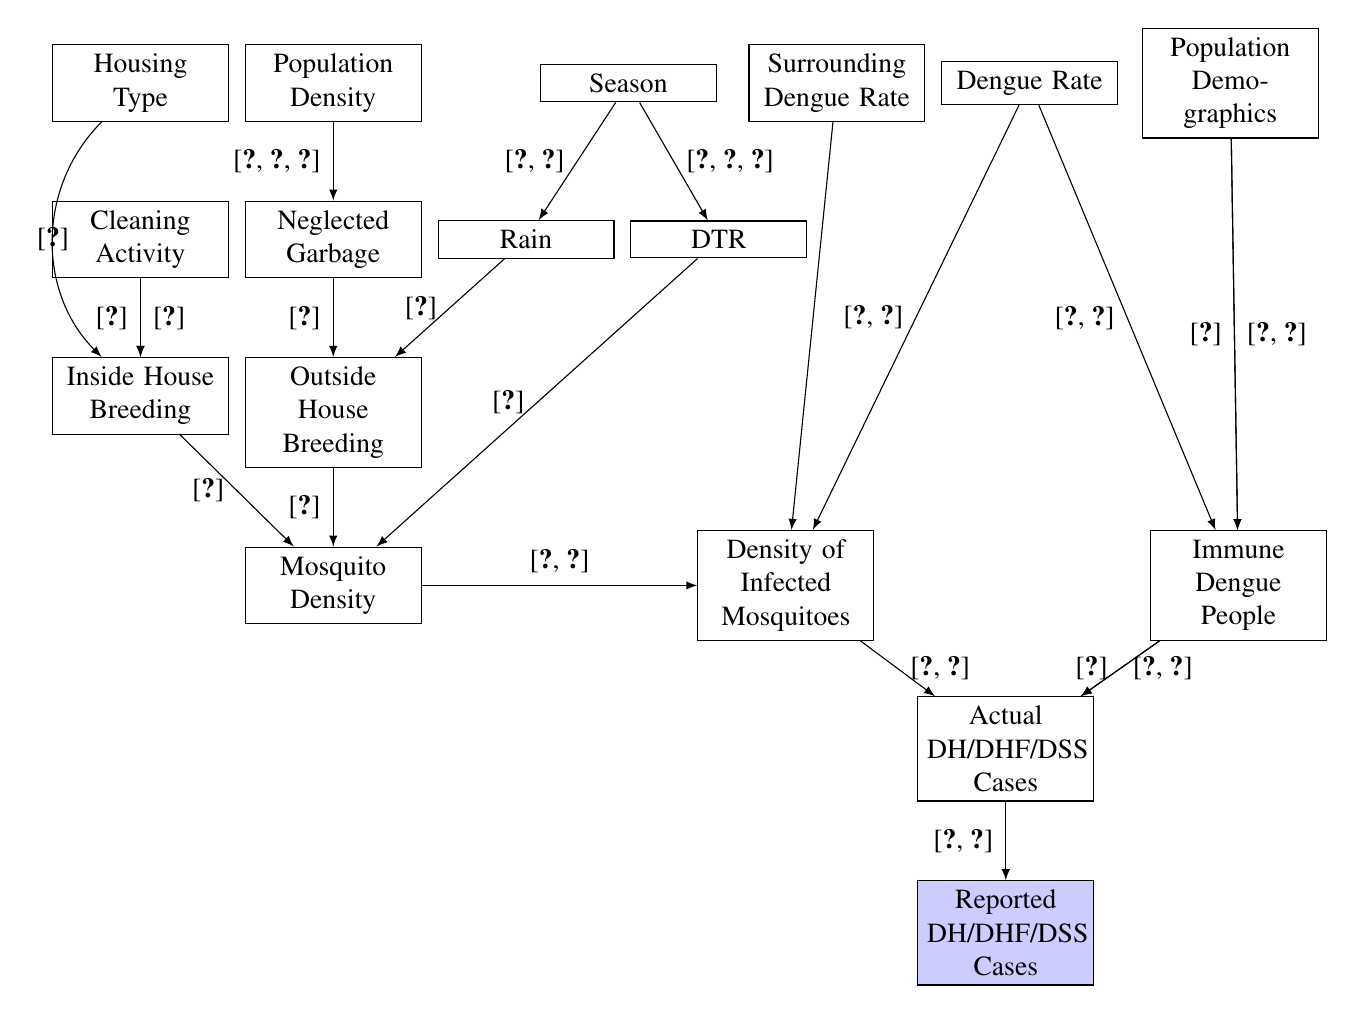
\begin{tikzpicture}[
	node distance=1cm and 0cm,
	mynode/.style={draw,  rectangle, text width=2cm,align=center}
	]
	
	
	\node[mynode] (pd) {Population Density};	
	\node[mynode, left = 0.2 cm of pd]  (ht){Housing Type};
	\node[mynode,below = of pd]  (grb){Neglected Garbage};
	\node[mynode,left = 0.2 cm of grb]  (ca){Cleaning Activity};
	\node[mynode,below =of grb]  (ob){Outside House Breeding};
	\node[mynode,below =of ca]  (ib){Inside House Breeding};
	\node[mynode,below  = of ob]  (md){Mosquito Density};
	
	\node[mynode, right = 1.5 cm of pd]  (season){Season};
	\node[mynode, below left = of season, right = 0.2 cm of grb]  (rain){Rain};
	\node[mynode, below right = of season, right = 0.2 cm of rain]  (DTR){DTR};
	
	
	
	\node[mynode, right = 0.4 cm of season]  (mndr){Surrounding Dengue Rate};
	\node[mynode, right = 0.2 cm of mndr]  (dr){Dengue Rate};
	\node[mynode, right = 0.3 cm of dr]  (pdr){Population Demographics};
	
	\node[mynode,right = 3.5 cm of md]  (dim){Density of Infected Mosquitoes};
	\node[mynode,right = 3.5 cm of dim]  (idp){Immune Dengue People};
	
	\node[mynode,below left = 1cm of idp]  (dh){Actual DH/DHF/DSS Cases};
	\node[mynode,below = of dh, fill=blue!20] (rdh){Reported DH/DHF/DSS Cases};
	
	
	\path (season) edge[-latex, ] node[left=1pt] {\cite{WPR2015, stoddard2014long}}   (rain)
	(season) edge[-latex] node[right=1pt] {\cite{lambrechts2011impact, carrington2013reduction, stoddard2014long}} (DTR)    
	(rain) edge[-latex]  node[left=1pt] {\cite{nakhapakorn2005information}} (ob)
	(DTR) edge[-latex] node[left=1pt] {\cite{lambrechts2011impact}}   (md)  
	(dr) edge[-latex] node[left=1pt] {\cite{adams2006cross, alto2008larval}} (idp)
	(pdr) edge[-latex] node[left=1pt]{\cite{whodenvsym2015}} (idp)
	(pdr) edge[-latex] node[right=1pt]{\cite{cummings2009impact,wilder2012denguetools}} (idp)
	(dr) edge[-latex]  node[left=1pt] {\cite{halstead2008dengue, esteva2000influence}} (dim)
	(mndr) edge[-latex] (dim)
	(ht) edge[-latex, bend right=45] node {\cite{favier2005influence}} (ib)
	
	(pd) edge[-latex]  node[left=1pt] {\cite{chang2009combining,knudsen1992vector,troyo2009urban}}   (grb)
	(grb) edge[-latex] node[left=1pt]{\cite{arunachalam2010eco}} (ob)
	(ob) edge[-latex] node[left=1pt] {\cite{sarfraz2014near}}  (md) 
	(ib) edge[-latex] node[left=1pt]{\cite{syarifah2008ovitrap}} (md) 
	(md) edge[-latex] node[above=1pt]{\cite{scott2003aedes, alto2008larval}} (dim)
	(dim) edge[-latex] node[right=1pt]{\cite{malavige2004dengue, chareonsook1999changing}}   (dh)
	(idp) edge[-latex] node[left=1pt]{\cite{whodenvsym2015}} (dh)
	(idp) edge[-latex] node[right=1pt]{\cite{ whitehorn2010dengue,reiter2010yellow}} (dh)
	(ca) edge[-latex] node[left=1pt]{\cite{chareonviriyaphap2003larval}} (ib)
	(ca) edge[-latex] node[right=1pt]{\cite{raju2008application}} (ib)
	(dh) edge[-latex] node[left=1pt]{\cite{wichmann2011dengue, bhatt2013global}} (rdh);
	
	\end{tikzpicture}

	\caption{Bayesian network model for the prediction of DH/DHF/DSS Cases. }
	\label{figure-bn_md_dr}
\end{figure}








\section*{References}

\bibliography{mybibfile}


\end{document}